% Do NOT change this "Section" title
% and do NOT add more "Section" level titles.
\section{Implementation}\label{sec:implementation}
\subsection{Software architecture}
To meet the software requirements it was decided to use Ada Tasks and Ada
Protected Objects. Protected objects are a special type of objects within Ada
to faciliate shared memory in a type safe way. As a requirement from the
customer was the use of the Ada Ravenscar profile. This profile restricts
the use of tasks to make the program easier to verify and validate. This meant
that each protected object in use was only allowed to be called from two
different tasks, no more.

The common data structure within the Naiad AUV is the CAN message structure,
it has a message ID and payload. These messages were modelled as objects within
the Sensor fusion code is the only data type that is passed around between
Ada Tasks.

To manage the incoming and outgoing data two tasks were set up for each link,
TCP\_IN and TCP\_OUT for the ethernet connection as well as CAN\_IN and CAN\_OUT for
the CAN bus connection. Each one of these tasks had only one responsibility, which
was to either send or receive CAN messages. Next task to be added was the Main
task which would do all the calculations. The design in this stage had five
different tasks with distinct responsibilty, though one main problem left to solve
was the requirement that in this design the Main task would have to do a lot of
filtering of CAN messages both to and from the TCP and CAN connection. To solve this
two new tasks were introduced the TCP\_IN\_FILTER and CAN\_IN\_FILTER. The filtering
tasks would be given a set of CAN message IDs on boot up that were of interest to
the Main task. The Main task had now only one responsibilty left and that was
to do the actual sensor fusion calculations.

\begin{figure}[ht]
    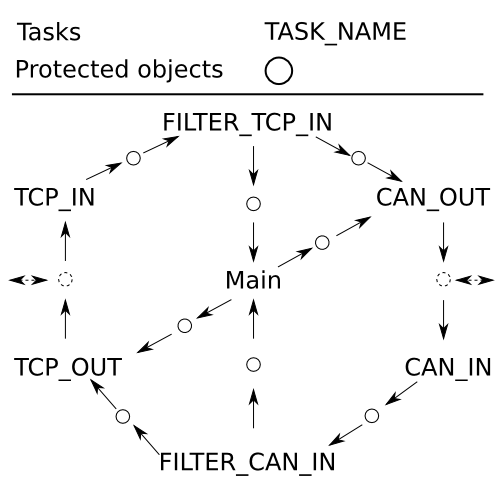
\includegraphics[width=0.5\textwidth]{./figure/software_architecture.png}
    \caption{Sensor fusion software architecture. Showing the different tasks and
    how they interact with each other through several different protected objects.}
    \label{fig:software_architecture}
\end{figure}

The final design of the software architecture is seen in figure \ref{fig:software_architecture}.
The dashed circles on the left and right side are protected objects specific for
the different hardware resources. For the CAN bus this is required because you
can't read and write at the same time but for the TCP connection multiple connections
can be done in parallell so it can be changed.


% You can use how many "subsections" and "subsubsections" you like.
\subsection{Sensor fusion calculations}
Text

% \subsubsection{Subsubsection1}
% Test of one column figure. It should be shown as close as possible to this
% text. If you can't see the figure its number is \ref{fig:one_column_figure}
% and located on page \pageref{fig:one_column_figure}.
% \begin{figure}[ht]
%     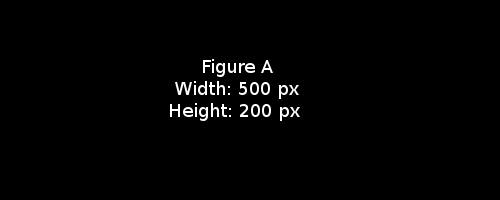
\includegraphics[width=0.5\textwidth]{./figure/figureA.png}
%     \caption{Figure A}
%     \label{fig:one_column_figure}
% \end{figure}
%
% \subsubsection{Subsubsection1}
% Test of two columns figure. It should be shown at the top of a page. If you
% can't see the figure its number is \ref{fig:two_column_figure}
% and located on page \pageref{fig:two_column_figure}.
% \begin{figure*}[t]
%     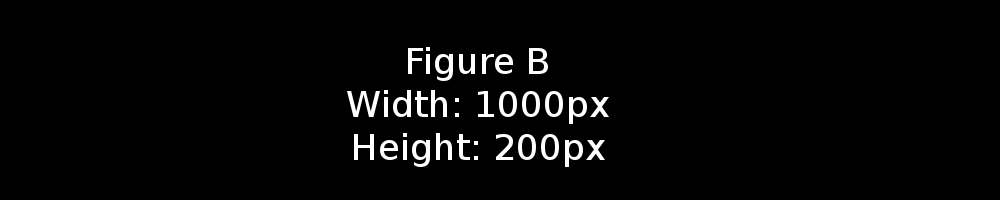
\includegraphics[width=1.0\textwidth]{./figure/figureB.png}
%     \caption{Figure B}
%     \label{fig:two_column_figure}
% \end{figure*}
